\section{E2: double descent}
\label{sec:dd}
\paragraph{Setup.} To see the whole curve, including the regime where the tree is too small to fit the data, the training set must be small relative to the largest tree. Every E2 run uses the first $n=2000$ CIFAR-10 (or Cats vs Dogs) training images, the ResNet-18 features projected onto their top 64 principal components (fitted on all training features, without labels), and a fraction of flipped labels (0\%, 10\% or 20\%). The tree has depth 2 (3 routers of width 4, 4 leaves) unless stated otherwise, and the leaf width $h$ is swept from 1 to 1024, which takes the tree from 1.1k to 308k parameters. Training is full-batch Adam for 4{,}000 steps with the squared loss, no weight decay and no early stopping. The test set is always the full, clean test set. Points are averages over 3 seeds (CIFAR-10, 0\% and 20\% noise), 2 seeds (Cats vs Dogs) or 1 seed (10\% noise and the largest width); shaded bands span the seeds.

\begin{figure}[!htbp]
\centering
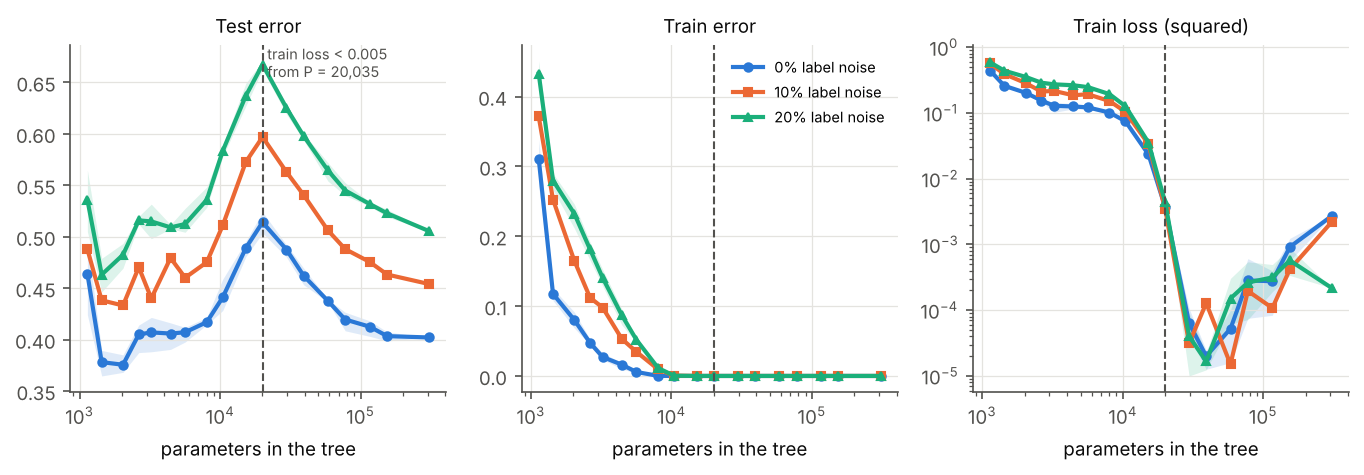
\includegraphics[width=\linewidth]{e2_width_cifar10.png}
\caption{CIFAR-10, model-wise double descent as the leaf width grows (depth 2, $n=2000$). Dashed line: the smallest tree whose final training loss is below 0.005. It coincides with $P=nK=20{,}000$. Training \emph{error} reaches 0 much earlier, at 8k to 10k parameters.}
\label{fig:width-c10}
\end{figure}

\paragraph{Model-wise double descent (Figure~\ref{fig:width-c10}).} On CIFAR-10 the test error follows the classical U-curve while the tree is small, then rises to a sharp peak where the training loss reaches zero, at $P\approx 20{,}000 = n\cdot K$ parameters (the number of numbers the tree has to fit), then falls again as the tree keeps growing:
\begin{center}\small
\begin{tabular}{lccc}
\toprule
label noise & best small tree & peak at $P\approx 20$k & largest tree (308k) \\
\midrule
0\% & 37.6\% (2.0k params) & 51.4\% & 40.2\% \\
10\% & 43.3\% (2.0k) & 59.7\% & 45.4\% \\
20\% & 46.3\% (1.4k) & 66.7\% & 50.5\% \\
\bottomrule
\end{tabular}
\end{center}
Label noise raises the peak (by 14, 16 and 20 points over the small-tree minimum) far more than it raises the rest of the curve, as reported for deep networks \cite{nakkiran2019}. The second descent is steep but, within the sizes we could afford, the largest tree does not beat the best small one on CIFAR-10.

\begin{figure}[!htbp]
\centering
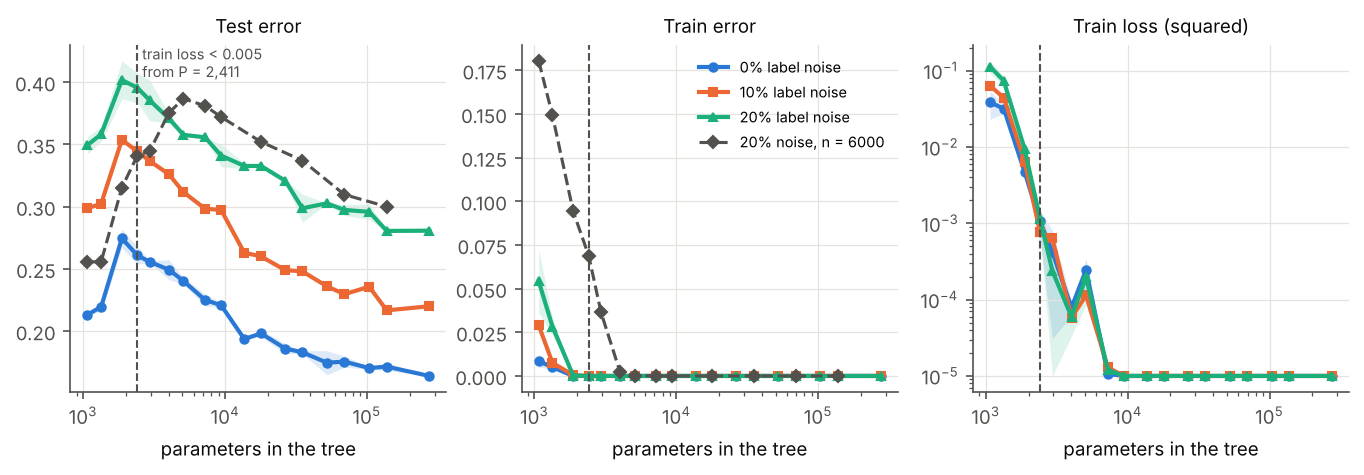
\includegraphics[width=\linewidth]{e2_width_catsdogs.png}
\caption{Cats vs Dogs, same setup ($K=2$). The peak is at about 2k parameters, where the training loss first drops below 0.005. Grey dashed: 20\% noise with $n=6000$ training images.}
\label{fig:width-cd}
\end{figure}

\paragraph{Cats vs Dogs (Figure~\ref{fig:width-cd}).} With two classes the tree reaches zero training loss already at about 2k parameters, so the first descent is short, but the peak and the long second descent are clear: test error goes from 21.3\% to a peak of 27.5\% and down to 16.4\% at 275k parameters (0\% noise), and from 34.9\% to 40.2\% and down to 28.1\% (20\% noise). Here the largest trees are the best. With three times as much data ($n=6000$, 20\% noise, grey curve) the peak moves right by about the same factor, to 5k--7k parameters (38.7\%); there, the smallest trees (25.6\%) beat every larger tree we trained.

\begin{figure}[!htbp]
\centering
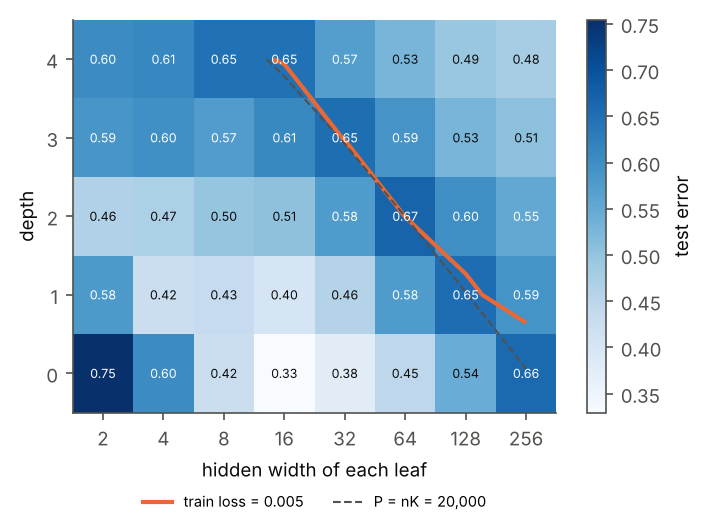
\includegraphics[width=0.62\linewidth]{e2_surface.png}
\caption{CIFAR-10, 20\% noise, test error over depth $\times$ leaf width (one seed). Orange: where the final training loss crosses 0.005. Dashed: trees with $P=20{,}000$ parameters. The worst cell of every row lies on these lines.}
\label{fig:surface}
\end{figure}

\paragraph{Width versus depth (Figure~\ref{fig:surface}).} A tree has two size knobs: how many leaves (depth) and how big each node is (width). We trained all 40 combinations of depth 0--4 and width 2--256. In every row, the worst test error (0.65 to 0.67) sits on the cell with $P\approx 14$k--23k parameters, and the interpolation contour and the line $P=nK$ run along the same diagonal of the grid. Whether parameters come from more leaves or wider leaves makes no difference to where the peak is: it is set by total size relative to $nK$. Adding leaves alone gives the same curve (Figure~\ref{fig:depth-samples}, left): with leaf width fixed at 16, test error goes from 33.2\% for a single network (depth 0, 1.2k parameters) up to 64.7\% at depth 4 (23k parameters, training loss $10^{-4}$) and back down to 48.6\% at depth 7 (189k parameters, 128 leaves).

\begin{figure}[!htbp]
\centering
\begin{minipage}{0.49\linewidth}\centering
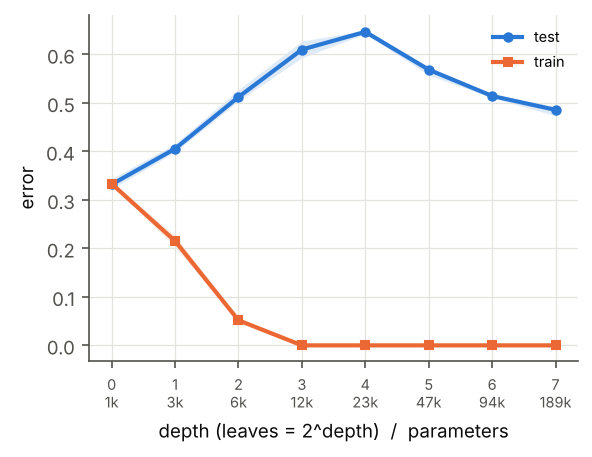
\includegraphics[width=\linewidth]{e2_depth.png}
\end{minipage}\hfill
\begin{minipage}{0.49\linewidth}\centering
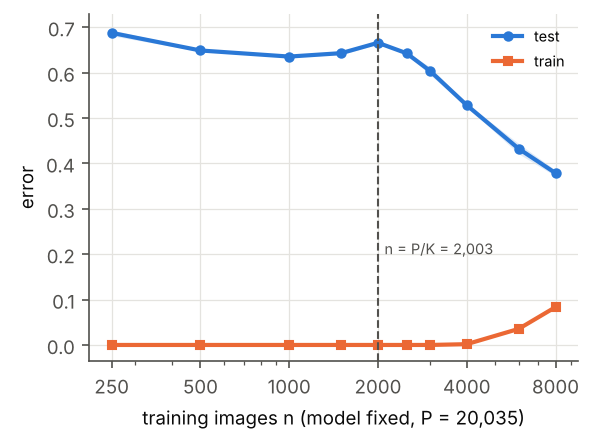
\includegraphics[width=\linewidth]{e2_samples.png}
\end{minipage}
\caption{Left: depth-wise sweep at leaf width 16 (20\% noise, 3 seeds); tick labels give depth and parameter count. Right: sample-wise sweep with the tree fixed at 20k parameters (20\% noise, 2 seeds).}
\label{fig:depth-samples}
\end{figure}

\paragraph{More data can hurt (Figure~\ref{fig:depth-samples}, right).} Holding the tree fixed at 20k parameters and growing the training set, test error first falls (68.7\% at $n=250$ to 63.5\% at $n=1000$), then rises to 66.6\% at $n=2000$, where $nK$ equals the parameter count, and only then falls steadily (37.8\% at $n=8000$). Doubling the data from 1000 to 2000 images makes this tree worse, because it moves the tree onto its interpolation point.

\begin{figure}[!htbp]
\centering
\begin{minipage}{0.49\linewidth}\centering
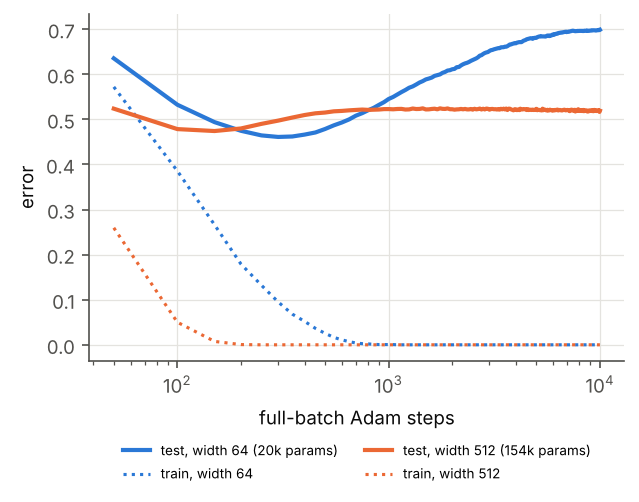
\includegraphics[width=\linewidth]{e2_epochs.png}
\end{minipage}\hfill
\begin{minipage}{0.49\linewidth}\centering
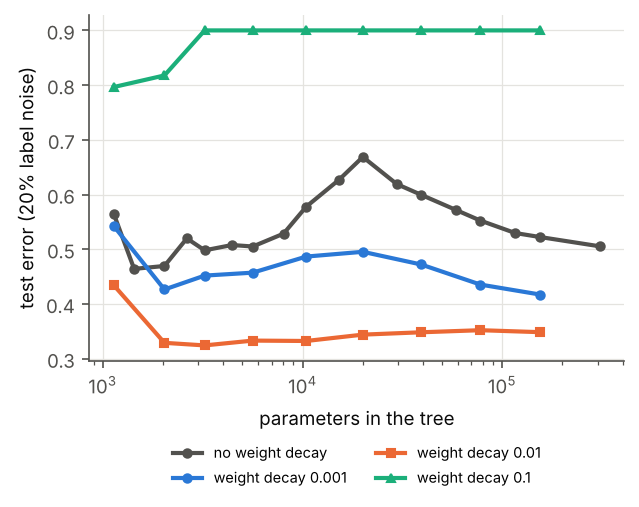
\includegraphics[width=\linewidth]{e2_wd.png}
\end{minipage}
\caption{Left: epoch-wise curves for a tree at the interpolation point (width 64) and well past it (width 512), 20\% noise. Right: the width sweep at 20\% noise with weight decay added (one seed).}
\label{fig:epochs-wd}
\end{figure}

\paragraph{Training time (Figure~\ref{fig:epochs-wd}, left).} We did \emph{not} see epoch-wise double descent. The tree at the interpolation point (width 64) reaches its best test error, 46.1\%, after 300 steps, while it still makes training errors; it then fits the flipped labels (zero training error from step 1{,}100) and its test error climbs to 66.9\% at step 4{,}000 and 69.9\% at step 10{,}000 as the training loss keeps shrinking. The wide tree (width 512) fits the training set by step 250, bottoms out at 47.4\%, and settles at 52\% with no further change. Two consequences: early stopping alone would erase the model-wise peak, and the height of the peak depends on how long training runs. Epoch-wise double descent in \cite{nakkiran2019} needed thousands of epochs of minibatch training on images; full-batch Adam on 64 fixed features may never enter the late regime where it appears.

\paragraph{Regularisation removes the peak (Figure~\ref{fig:epochs-wd}, right).} With weight decay $10^{-3}$ the peak at 20k parameters drops from 66.7\% to 49.5\%. With $10^{-2}$ there is no peak at all: test error stays between 32.4\% and 35.2\% for every width from 4 upwards (43.4\% at width 1), far better than any unregularised tree in the width sweep. These trees never drive the training loss to zero (it stays above 0.13), even at widths where they classify almost every training image as labelled. With $10^{-1}$ every tree collapses to a constant prediction (90\% error). This matches the result of Nakkiran et al.\ \cite{nakkiran2020} that well-tuned regularisation makes test error fall monotonically with size; double descent is a property of unregularised (or weakly regularised) training to zero loss.

\begin{figure}[!htbp]
\centering
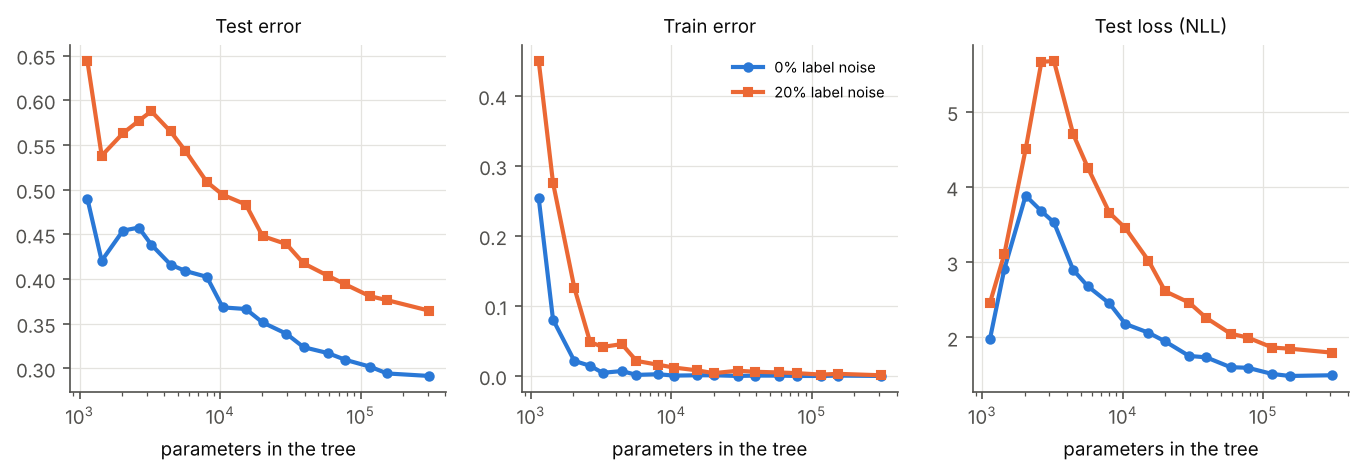
\includegraphics[width=\linewidth]{e2_width_cifar10_ce.png}
\caption{The CIFAR-10 width sweep with the mixture (cross-entropy) loss instead of the squared loss (one seed). The peak moves to about 3k parameters and is clearest in the test loss.}
\label{fig:ce}
\end{figure}

\paragraph{Cross-entropy (Figure~\ref{fig:ce}).} With the mixture loss the peak moves left, to 2.6k to 3.2k parameters, and is smaller in test error (from 42.0\% to 45.8\% with clean labels, from 53.8\% to 58.8\% with 20\% noise) but large in test loss. Past it, test error falls all the way to 29.4\% (clean) and 36.5\% (20\% noise) for the largest trees, much lower than with the squared loss. Cross-entropy only needs the correct class to win, so far fewer parameters suffice to fit every label, and the trees reach the second descent sooner.
